\documentclass[12pt,hyperref,]{ctexart}
\usepackage{lmodern}
\usepackage{amssymb,amsmath}
\usepackage{ifxetex,ifluatex}
\usepackage{fixltx2e} % provides \textsubscript
\ifnum 0\ifxetex 1\fi\ifluatex 1\fi=0 % if pdftex
  \usepackage[T1]{fontenc}
  \usepackage[utf8]{inputenc}
\else % if luatex or xelatex
  \ifxetex
    \usepackage{xltxtra,xunicode}
  \else
    \usepackage{fontspec}
  \fi
  \defaultfontfeatures{Mapping=tex-text,Scale=MatchLowercase}
  \newcommand{\euro}{€}
\fi
% use upquote if available, for straight quotes in verbatim environments
\IfFileExists{upquote.sty}{\usepackage{upquote}}{}
% use microtype if available
\IfFileExists{microtype.sty}{%
\usepackage{microtype}
\UseMicrotypeSet[protrusion]{basicmath} % disable protrusion for tt fonts
}{}
\usepackage[left=2.5cm,right=2.5cm,top=2.5cm,bottom=2.5cm]{geometry}
\ifxetex
  \usepackage[setpagesize=false, % page size defined by xetex
              unicode=false, % unicode breaks when used with xetex
              xetex]{hyperref}
\else
  \usepackage[unicode=true]{hyperref}
\fi
\usepackage[usenames,dvipsnames]{color}
\hypersetup{breaklinks=true,
            bookmarks=true,
            pdfauthor={管晓倩; 王瑶; 杨洁; 张莉},
            pdftitle={武汉市疫情预测分析},
            colorlinks=true,
            citecolor=blue,
            urlcolor=blue,
            linkcolor=magenta,
            pdfborder={0 0 0}}
\urlstyle{same}  % don't use monospace font for urls
\usepackage{longtable,booktabs}
\setlength{\emergencystretch}{3em}  % prevent overfull lines
\providecommand{\tightlist}{%
  \setlength{\itemsep}{0pt}\setlength{\parskip}{0pt}}
\setcounter{secnumdepth}{5}

\title{武汉市疫情预测分析}
\author{管晓倩 \and 王瑶 \and 杨洁 \and 张莉}
\date{}



% Redefines (sub)paragraphs to behave more like sections
\ifx\paragraph\undefined\else
\let\oldparagraph\paragraph
\renewcommand{\paragraph}[1]{\oldparagraph{#1}\mbox{}}
\fi
\ifx\subparagraph\undefined\else
\let\oldsubparagraph\subparagraph
\renewcommand{\subparagraph}[1]{\oldsubparagraph{#1}\mbox{}}
\fi

\begin{document}
\maketitle
\begin{abstract}
2019年12月湖北武汉陆续发现多例新型冠状病毒肺炎(COVID-19),因病毒显著的人传人特性致使其伴随着高度且密集的人口流动迅速蔓延,构成了全球突发公共卫生事件。本研究基于海外检测到的病例数并结合敏感性分析估计武汉市封城时的感染人数。除此之外,稍作调整的SEIR模型预测的武汉市疫情高峰期在2月20号左右。从结果中可以发现,在严格的防控措施下疫情得到了有效抑制,验证了目前防控措施的有效性。
\end{abstract}

\hypertarget{ux5f15ux8a00}{%
\section{引言}\label{ux5f15ux8a00}}

\hypertarget{ux80ccux666fux53caux7814ux7a76ux610fux4e49}{%
\subsection{背景及研究意义}\label{ux80ccux666fux53caux7814ux7a76ux610fux4e49}}

2019年12月,湖北武汉陆续发现多例新型冠状病毒肺炎(coronavirus~disease~2019,COVID-19),因病毒显著的人传人特性致使其伴随着高度且密集的人口流动迅速蔓延,构成了全球突发公共卫生事件。为控制疫情,1月23日武汉市``封城'',离汉通道关闭,全国各省市相继启动突发公共卫生事件Ⅰ级应急响应,春节假期延长,部分社会活动停止。

截至2020年5月12日24时,我国累计确诊病例82926例,治愈出院78189例,死亡达4633例。疫情的爆发,除了疫情自身所带来的疾病损害、病例死亡外,还会引起极大的社会恐慌,并造成巨大的经济损失,严重威胁人类健康与社会发展。

本次研究主要利用SEIR模型和改进的SEIR模型对武汉新冠病毒的疫情发展进行建模和预测。

\hypertarget{ux7814ux7a76ux601dux8def}{%
\subsection{研究思路}\label{ux7814ux7a76ux601dux8def}}

本文主要分析武汉市疫情,整体可主要分为以下四个部分:
第一章:绪论。首先介绍了文章研究的背景和意义,说明了研究的必要性。然后介绍数据和相关资料的来源。最后,简要说明了本文的框架和研究所使用的方法。
第二章:描述统计。这部分通过图表直观展现疫情的具体情况以及疫情对社会经济产生的影响,为下文的实证研究奠定了基础。
第三章:实证分析。这部分主要包括SEIR等模型的介绍,武汉封城时感染人数估计和疫情高峰期预测。
第四章:结论与建议。根据实证分析的结果得出主要结论并提出可供政府参考的意见和措施。

\hypertarget{ux7814ux7a76ux65b9ux6cd5}{%
\subsection{研究方法}\label{ux7814ux7a76ux65b9ux6cd5}}

本文主要使用以下两种种方法进行研究:
一、描述统计方法。运用制表和分类,图形以及计算概括性数据来描述全国以及武汉市的疫情情况。
二、传染病模型分析。文章基于武汉市1月20日---6月1日疫情数据,利用SEIR模型和SEIDC模型对武汉市疫情情况进行分析。

\hypertarget{ux6570ux636eux6765ux6e90}{%
\subsection{数据来源}\label{ux6570ux636eux6765ux6e90}}

本文收集武汉市1月20---6月1日的数据,包括累计确诊人数,累计治愈人数和累计死亡人数。数据主要来源:国家卫生健康委员会(\url{http://www.nhc.gov.cn/}),湖北省卫生健康委员会---通知公告(\url{http://wjw.hubei.gov.cn/fbjd/tzgg/}),武汉市卫生健康委员会---防控要闻(\url{http://wjw.wuhan.gov.cn/ztzl_28/fk/flfg/)和国家统计局(http://www.stats.gov.cn/})。还有部分实时更新数据来自:(\url{https://github.com/839Studio/Novel-Coronavirus-Updates})。

\hypertarget{ux7406ux8bbaux65b9ux6cd5}{%
\section{理论方法}\label{ux7406ux8bbaux65b9ux6cd5}}

\hypertarget{ux8f6eux5ed3ux4f3cux7136ux4f30ux8ba1ux6cd5}{%
\subsection{轮廓似然估计法}\label{ux8f6eux5ed3ux4f3cux7136ux4f30ux8ba1ux6cd5}}

在目标参数呈非正态分布时,如果计算基于正态分布的WaldCI型置信区间来计算模型中某个参数的置信区间将会产生偏差,
尤其在无法计算目标参数的标准误时,该置信区间也无法计算。而轮廓似然置信区间是基于卡方分布且无需计算标准误,构造置信区间依据的是似然比检验。因此,能够解决参数不服从正态分布和标准误无法计算时置信区间的计算问题。

\hypertarget{ux654fux611fux6027ux5206ux6790ux65b9ux6cd5}{%
\subsection{敏感性分析方法}\label{ux654fux611fux6027ux5206ux6790ux65b9ux6cd5}}

最简单和最常见的方法之一是每次更改一个因素(One-at-a-tim,OAT),以查看这会对输出产生什么影响。OAT通常包括:移动一个输入变量,保持其他变量的基线值,然后以相同的方式对每个其他输入进行重复。将所有其他变量固定在它们的基线值上,通过每次更改一个变量,可以增加结果的可比较性。

\hypertarget{seirux6a21ux578bux4f30ux8ba1}{%
\subsection{SEIR模型估计}\label{seirux6a21ux578bux4f30ux8ba1}}

SEIR传染病模型主要将人群分为四个部分,即易感者S、潜伏者E、感染者I和康复者R。SEIR模型的基本应用没有考虑人群流入或流出,应用中考虑了公式的少许调整,包括将接触感染者被感染的情况分为接触潜伏期患者被感染和接触感染者被感染两种情况,并对于感染者不仅考虑其康复的概率,也将少部分患者死亡的可能性也考虑在其中。在后续的模型改进研究中,引入了迁入与迁出两部分加以考虑。

\hypertarget{ux63cfux8ff0ux7edfux8ba1}{%
\section{描述统计}\label{ux63cfux8ff0ux7edfux8ba1}}

\hypertarget{ux5404ux533aux57dfux7b49ux7ea7ux65b0ux51a0ux80baux708eux57faux672cux60c5ux51b5}{%
\subsection{各区域等级新冠肺炎基本情况}\label{ux5404ux533aux57dfux7b49ux7ea7ux65b0ux51a0ux80baux708eux57faux672cux60c5ux51b5}}

\begin{figure}
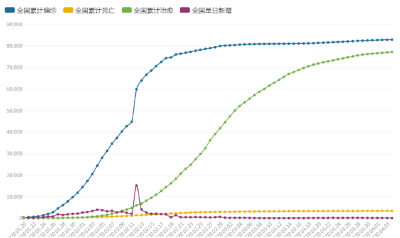
\includegraphics[width=5.56in]{image/3.1.1} \caption{全国新冠肺炎基本情况}\label{fig:3.1}
\end{figure}

\begin{figure}
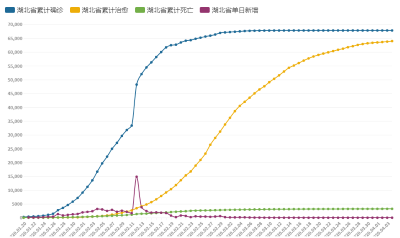
\includegraphics[width=5.56in]{image/3.1.2} \caption{湖北省新冠肺炎基本情况}\label{fig:3.2}
\end{figure}

\begin{figure}
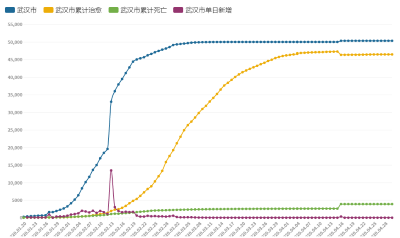
\includegraphics[width=5.56in]{image/3.1.3} \caption{武汉市新冠肺炎基本情况}\label{fig:3.3}
\end{figure}

全国,湖北省,以及武汉市三个不同等级区域的趋势图分别如图所示。通过对比发现其基本趋势是一致的,因为全国的大部分病例都集中在湖北,湖北病例又最多发生在武汉。所以对武汉市做疫情预测分析是具有实际意义的。

从图中可以看出,在二月二十日之前,各地区累计确诊病例和单日新增病例增长的速度都是较快的,基本上是呈一个陡坡式增长,此时疫情处于发展期。二月末至三月初,增长趋势开始显著减缓。三月初以后,基本趋于缓和。此趋势即为全国疫情发展的基本情况。同时,图中所示拐点皆为二月十二日,当日全国新增15152例,其中武汉市有13436名。由于当日将临床诊断也记为确诊,所以出现暴增。

\hypertarget{ux6b66ux6c49ux5e02ux4ebaux53e3ux6d41ux51faux72b6ux51b5ux5206ux6790}{%
\subsection{武汉市人口流出状况分析}\label{ux6b66ux6c49ux5e02ux4ebaux53e3ux6d41ux51faux72b6ux51b5ux5206ux6790}}

武汉市是中部地区的中心城市和长江经济带核心城市,也是重要的交通枢纽和教育重市,其每年的流动人口超过500万人。本次新冠肺炎最先发生在武汉,且全国各省市发现的绝大部分病例都与都与武汉有关。疫情爆发之初正值春运期间,人口流动很大而疫情的大范围扩散与人口流动密切相关,对武汉虎人口流动与相关疫情进行回顾性分析,有利于总结经验,做好今后的流行性疾病防控工作。

\begin{figure}
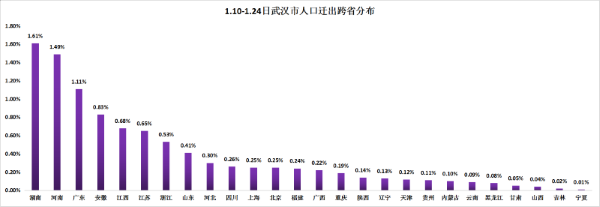
\includegraphics[width=8.33in]{image/3.2.1} \caption{武汉市人口迁出跨省分布}\label{fig:3.4}
\end{figure}

\begin{figure}
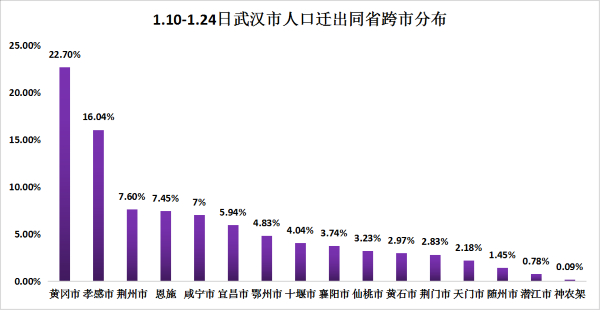
\includegraphics[width=8.33in]{image/3.2.2} \caption{武汉市人口迁出同省跨市分布}\label{fig:3.5}
\end{figure}

\begin{figure}
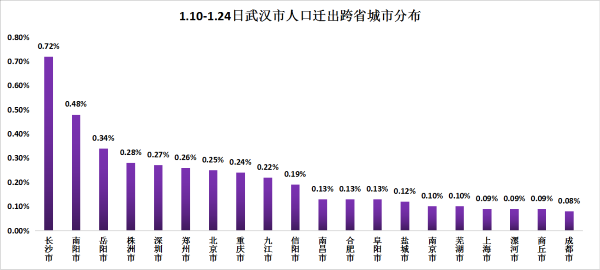
\includegraphics[width=8.33in]{image/3.2.3} \caption{武汉市人口迁出跨省跨市分布}\label{fig:3.6}
\end{figure}

武汉市人口跨省流动、同省跨市流动和跨省跨市流动分别由图所示,数据来源于百度迁徙平台。武汉市流出人口以省内流动为主,约占总流出人口的89.91\%,而跨省流出中五成以上流入湖南,河南,广东,安徽,江西五省,基本都是湖北邻省。在省内跨市流动中,武汉市流动人口最多流入黄冈和孝感两市,分别占总流出人口的22.7\%和16.04\%;跨省跨市流动中,五成以上流入长沙、南阳、岳阳,株洲、深圳、郑州、北京、重阳、九江、信阳十市,长沙和南阳比例最高,分别为0.72\%和0.48\%。

\hypertarget{ux6b66ux6c49ux5e02ux4ebaux53e3ux6d41ux51faux5bf9ux75abux60c5ux6269ux6563ux8513ux5ef6ux7684ux5f71ux54cd}{%
\subsection{武汉市人口流出对疫情扩散蔓延的影响}\label{ux6b66ux6c49ux5e02ux4ebaux53e3ux6d41ux51faux5bf9ux75abux60c5ux6269ux6563ux8513ux5ef6ux7684ux5f71ux54cd}}

\begin{figure}
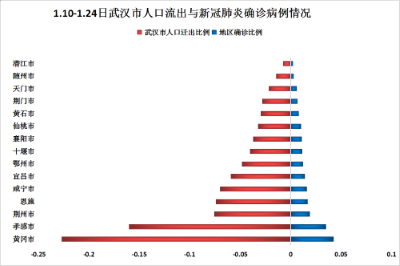
\includegraphics[width=5.56in]{image/3.3.1} \caption{武汉市人口流出与湖北省内新冠肺炎确诊情况}\label{fig:3.7}
\end{figure}

\begin{figure}
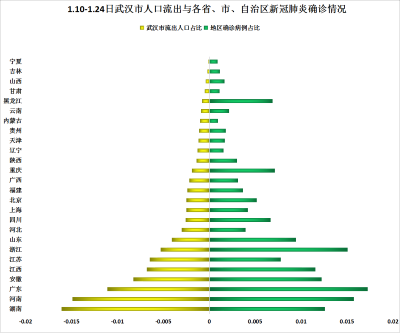
\includegraphics[width=5.56in]{image/3.3.2} \caption{武汉市人口流出与各省、市、自治区新冠肺炎确诊情况}\label{fig:3.8}
\end{figure}

由图可知,在省内跨市流动中,人口流入最多的黄冈、孝感两地已经占了省内确诊的三成以上,其他城市的确诊比例基本都与流入比例正向相关。所以说,从湖北省内看,武汉市人口的主要流向地与疫情发展状况高度相关。而在省外流动中,武汉人口流出与较为严重的省份大致对应,流入人口靠前的省份疫情确诊数量基本也在前列,多集中在东部中部与湖北相邻的省份。武汉市流出人口排名前三的湖南省、河南省、广东省,其确诊比分比为1.258\%、1.573\%和1.724\%,是除湖北省外确诊排名前三的省份。而流入比例相对不高的黑龙江等地确诊比例较高,说明该地可能发生二次感染的情况较为严重。

\hypertarget{ux75abux60c5ux4e0bux7684ux7ecfux6d4eux53d8ux5316ux8d8bux52bf}{%
\subsection{疫情下的经济变化趋势}\label{ux75abux60c5ux4e0bux7684ux7ecfux6d4eux53d8ux5316ux8d8bux52bf}}

\begin{figure}
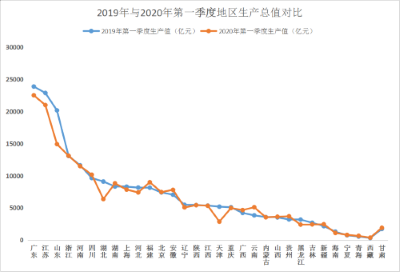
\includegraphics[width=5.56in]{image/3.4.1} \caption{2019-2020年第一季度地区生产总值对比图}\label{fig:3.9}
\end{figure}

大部分省市2020年的GDP水平都低于上年同季度,其中以湖北省下降的的比例最为显著。根据地区生产总值统一核算结果,2020年一季度,武汉市GDP按可比价格计算,比上年同期下降40.5\%。其中,第一产业增加值下降36.4\%,第二产业增加值45.4\%,第三产业增加值下降37.7\%。

\begin{figure}
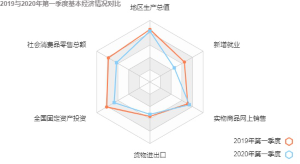
\includegraphics[width=4.17in]{image/3.4.2} \caption{2019-2020年第一季度经济情况对比图}\label{fig:3.10}
\end{figure}

雷达图显示的国民经济各方面指标指出,除了实物商品网上销售以外,各个指标都有一定程度的较少,因为减少出门的几率人们会选择网购来购买必须的生活物资。数据显示,一季度按可比价格计算,国内生产总值同比下降6.8\%;社会消费品零售总额同比下降19\%;全国固定资产投资同比下降16.1\%;货物进出口总额下降6.4\%。

\hypertarget{ux5b9eux8bc1ux5206ux6790}{%
\section{实证分析}\label{ux5b9eux8bc1ux5206ux6790}}

\hypertarget{ux6b66ux6c49ux5e02ux5c01ux57ceux65f6ux75abux60c5ux60c5ux51b5ux4f30ux8ba1}{%
\subsection{武汉市封城时疫情情况估计}\label{ux6b66ux6c49ux5e02ux5c01ux57ceux65f6ux75abux60c5ux60c5ux51b5ux4f30ux8ba1}}

\hypertarget{ux7814ux7a76ux80ccux666f}{%
\subsubsection{研究背景}\label{ux7814ux7a76ux80ccux666f}}

由于武汉市内的疫情数据存在着缺失,用来估计封城时武汉市的患病数存在着一定的误差,故使用海外检测到的病例数来估计在封城之前在武汉可能发生的病例更具有可靠性。现有背景如下:
武汉市于2020年1月23日凌晨2时``封城'';在``封城''之前,官方的确诊病例数仅是300多,但是在1月29日官方的确诊病例数已经上升到了2000例左右;武汉市人口1100万,武汉国际机场的人流量是1900万;在2019年11月以及12月的两个月里,每天从武汉国际机场出发的国际旅行平均总次数为3301次;截至1月22日,在中国大陆以外发现8例,均从武汉出发的病例;截至1月29日,在中国大陆以外发现67例。

\hypertarget{ux57faux672cux5047ux8bbe}{%
\subsubsection{基本假设}\label{ux57faux672cux5047ux8bbe}}

本次研究共设有两方面的假设,首先是基于流行病的假设:估计不包括症状轻微或无症状的病例;平均潜伏期6天,从症状出现到检测出的平均时间4天。其次基于统计学的假设:武汉市的``海外病例''和``确诊病例''之间存在独立关系;来自武汉的海外检测到的病例数是服从二项分布的,其中p是任一病例在海外被检测到的概率,这个假设只影响区间估计;国际旅行者与暴露于新型冠状病毒以及被感染的风险无关。

\hypertarget{ux4f30ux8ba1ux6b66ux6c49ux5e02ux5c01ux57ceux65f6ux7684ux75abux60c5ux60c5ux51b5}{%
\subsubsection{估计武汉市封城时的疫情情况}\label{ux4f30ux8ba1ux6b66ux6c49ux5e02ux5c01ux57ceux65f6ux7684ux75abux60c5ux60c5ux51b5}}

通过下述式子对1月22日以及1月29日且来自武汉的海外检测到的病例数,来估计封城前武汉的潜在病例数,利用轮廓似然估计法求得置信区间,最后进行敏感性分析以得到不同参数相对于基线的变化情况。

1.总的武汉病例数=海外检测到的病例数/海外发现任一病例的可能性;

2.海外发现任一病例的可能性=国际旅行的每日概率*发现病例的平均时间;

3.国际旅行的每日概率 =
2019年11月至12月每天从武汉出发的国际旅客/武汉国际机场的人流量;

4.发现病例的平均时间=潜伏期的平均时间+从症状出现到检测出的平均时间。

\hypertarget{ux4f30ux8ba1ux7ed3ux679c}{%
\subsubsection{估计结果}\label{ux4f30ux8ba1ux7ed3ux679c}}

估计出的具体结果以及敏感性分析的结果如下表所示,敏感性分析中分别改变了人流量以及检测时间这两个参数,当人流量更少时,估计出的确诊患者数会大大减少,当检测时间更短时,估计出的确诊患者数相比于基线情况会增加。敏感性分析中参数的改变反应了可能的不确定,基于1月29日的数据估计出的结果更具有说服力,因为到1月29日时大多数的来自武汉的境外病例已经被检测到了。基于1月29日的海外检测到来自武汉的病例数,估计出封城时可能存在的患者数为38564人,考虑到漏报的数据,数据收集时存在问题以及出口筛查可能减少了``海外病例数'',国际旅行者可能更富有,接触的风险更低等问题,这里的估计结果只是一个可能的值。

\begin{verbatim}
                           表1 武汉市病例数估计
\end{verbatim}

\begin{longtable}[]{@{}ccccc@{}}
\toprule
& 基线 & 更少的人流量 & 更少的检测时间 &\tabularnewline
\midrule
\endhead
从武汉国际机场出发的每日旅客数 & 3301 & 3301 & 3301 &\tabularnewline
武汉国际机场的人流量 & 19 million & 11 million & 19 million
&\tabularnewline
检测时间 & 10天 & 10天 & 8天 &\tabularnewline
基于1月22日数据估计的总病例数 & 4605 & 2666 & 5756 &\tabularnewline
基于1月22日估计的总病例数(95\%CI) & (2100, 8550) & (1220, 4940) & (2630,
10700) &\tabularnewline
基于1月29日估计的总病例数 & 38564 & 22327 & 48205 &\tabularnewline
基于1月29日估计的总病例数(95\%CI) & (30000, 48470) & (17340, 28030) &
(37510, 60600) &\tabularnewline
\bottomrule
\end{longtable}

\hypertarget{ux6b66ux6c49ux5e02ux75abux60c5ux9ad8ux5cf0ux9884ux6d4b}{%
\subsection{武汉市疫情高峰预测}\label{ux6b66ux6c49ux5e02ux75abux60c5ux9ad8ux5cf0ux9884ux6d4b}}

\hypertarget{ux57faux7840seirux6a21ux578bux7684ux5e94ux7528}{%
\subsubsection{基础SEIR模型的应用}\label{ux57faux7840seirux6a21ux578bux7684ux5e94ux7528}}

SEIR基本模型使用的基本参数主要来源于文献的参考,包括感染率、发病率、康复率以及死亡率等,初始模型考虑的是在封城的情况下,认为不存在迁入与迁出对未来情况的预测。

按照基本预测,潜伏期患者的数量会在封城后第40天达到最大,感染者的人数大约在90天后达到最大,而康复者的数量一直在缓慢上升,在预测的时间都没有达到基本稳定的状态,即疫情在长时间内得不到稳定控制。这里认为出现这种情况的主要原因是刚刚封城时期尽管采取了一定的措施,但力度不足,传染速度较快而康复速度较慢。因此按照这种情况进行估计,预测结果也会更加严重,潜伏期和感染者的预测数量都会较多,并且康复情况的预期也会较为缓慢。

由于后期应对措施的逐渐增加,康复速度加快,在拐点处将预测分为前后两部分,按照真实情况的数据分别估计这两部分的治愈率r和死亡率d。可以看到按照前一阶段的情况,潜伏期患者依旧会在40天的时候达到最大,而感染者的数量较少,这可能是由于前期疫情突然,数据不够完整,感染者确诊不够迅速准确。而康复者的数量在预测期间依旧没有达到平稳状态,也就是说在这一预测下,大部分人康复需要更久。

\begin{figure}
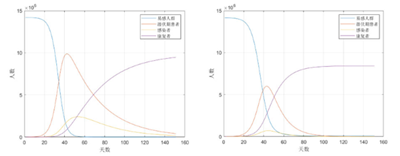
\includegraphics[width=5.56in]{image/4.2.1} \caption{拟合r、d后的SEIR(左:前期,右:后期)}\label{fig:1}
\end{figure}

根据二月中旬之后的情况进行预测来看,潜伏期患者和感染者的最高人数都明显更少,当然事实上这一预测的人数是少于实际情况的,因为这时的康复率较高,各方面应对更加及时,由于出行限制,传染概率也有所降低,没有包含前面时间传染率高而康复率低的情况。从这一预测也可以看到,大约在第70天康复人数达到最高并基本趋于稳定,即这时大部分患者都得以康复,疫情基本得到控制。

\hypertarget{seirux6a21ux578bux7684ux6539ux8fdb}{%
\subsubsection{SEIR模型的改进}\label{seirux6a21ux578bux7684ux6539ux8fdb}}

接下来我们通过引入迁入In和迁出Out来调整原始m模型,动态展现易感人群S的变动状态。

\begin{figure}
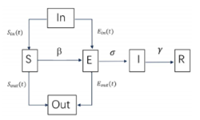
\includegraphics[width=2.78in]{image/4.2.2} \caption{加入迁入、迁出的SEIR模型}\label{fig:2}
\end{figure}

修改后的模型表示为:

\begin{figure}
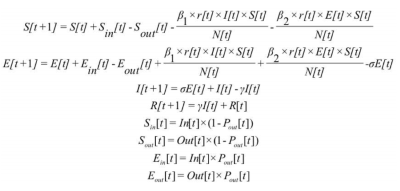
\includegraphics[width=5.56in]{image/fom} \caption{改进的SEIR模型}\label{fig:3}
\end{figure}

为了应用模型,需要估计参数贝塔和伽马。其中传染系数贝塔是感染者每天接触的人数k和传染概率b的乘积。根据对数据的拟合,可以得到b的估计,根据确诊者与潜伏期患者可能接触到的人数不同,确诊者进行隔离从而每日接触人数更少,因此参考相关文献,设置确诊者与潜伏期患者每日接触人数的不同值,可以得到不同情况的β值。

根据政策的逐渐提出和完善,如出行的限制会减少病毒传播的可能,可以对接触人数进行不同的设置,从而得到不同的贝塔加入模型进行拟合。对于每日累计康复人数和感染人数进行计算,结果取平均值进行康复率的估计。根据参数的设定进行模型构造,得到如下结果:

\begin{figure}
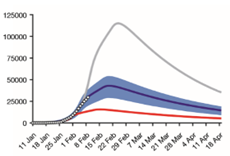
\includegraphics[width=3.19in]{image/4.2.3} \caption{加入迁入、迁出的SEIR模型结果}\label{fig:4}
\end{figure}

图为SEIR模型预测的结果,蓝色线为根据现有情况的预测结果,可以看到确诊人数在2月20日左右达到顶峰,这里对武汉b部分地区开始隔离控制出行这一政策时间的前后差别进行了预测分析,灰色曲线为这一政策实施推后5天的情况预测,这样确诊人数的预测会翻倍增长,而红色曲线为政策提前5天实施的情况估计,在这样的情况下,确诊人数会大量减少。可以看到虽然政策并不算在最早的时刻开始实施,但在当时的情况下,已经及时地减少了更大面积的病毒传播。

\hypertarget{ux8ba8ux8bba}{%
\section{讨论}\label{ux8ba8ux8bba}}

对武汉市的情况而言,感染者人数在2月前期增长最为迅速,在2月20日左右达到最高,这一时期往后,恢复率开始上升,总患病人数逐渐下降,预计在4月底往后,大部分感染者已经可以得到恢复。

为统筹疫情防控和经济社会发展,营造安全健康的生活环境,武汉在全市范围内开展了核酸检测,全市未进行过新冠病毒核酸检测的常住居民和暂住居民均纳入本次检测范围。本次检测人数达到989万人以上,检出无症状感染者300名,追踪密切接触者1174名,结果均为阴性,并对无症状感染者和密切接触者均进行了医学隔离观察,没有发现无症状感染者传染他人的情况,没有发现确诊病例。截止6月4日24时,武汉市确诊病例以及疑似病例均得到清零。

\hypertarget{ux81f4ux8c22}{%
\section*{致谢}\label{ux81f4ux8c22}}
\addcontentsline{toc}{section}{致谢}

感谢曹盛力、蔡洁等的研究结果为我们提供了思路加深了我们对研究方法的理解,并且感谢闫军老师的课程提高了了我们对于软件以及模型方法的学习使用。

\hypertarget{ux53c2ux8003ux6587ux732e}{%
\section*{参考文献}\label{ux53c2ux8003ux6587ux732e}}
\addcontentsline{toc}{section}{参考文献}

{[}1{]}
曹盛力,冯沛华,时朋朋.修正SEIR传染病动力学模型应用于湖北省2019冠状病毒病(COVID-19)疫情预测和评估{[}J{]}.浙江大学学报(医学版),2020,49(02):178-184.

{[}2{]}
蔡洁,贾浩源,王珂.基于SEIR模型对武汉市新型冠状病毒肺炎疫情发展趋势预测{[}J{]}.山东医药,2020,60(06):1-4.

{[}3{]} 韩栋,陈征,陈平雁,Nakamura
Tsuyoshi.轮廓似然函数及其应用{[}J{]}.中国卫生统计,2012,29(04):478-480+483.

{[}4{]}
许小可,文成,张光耀,等.新冠肺炎爆发前期武汉外流人口的地理去向分布及影响{[}J/OL{]}.电子科技大学学报,1-6{[}2020-03-11{]}.

{[}5{]}
张琳.新冠肺炎疫情传播的一般增长模型拟合与预测{[}J/OL{]}.电子科技大学学报
,1-4{[}2020-03-11{]}.

{[}6{]} BECKER NG, GLASS K, LI Z, et al.~Controlling emerging infectious
diseases like SARS{[}J{]}.Math biosci, 2005, 193(2):205-221.

{[}7{]} 戴应基,曾文霞. SARS 流行状况及预防{[}J{]}. 旅行医学科学, 2004,
10(4):43-47.

{[}8{]} 范如国,王奕博,罗明,等. 基于 SEIR
的新型肺炎传播模型及拐点预测分析{[}J/OL{]}. 电子科技大学学报,
1-6{[}2020-03-7{]}.

\end{document}
